\chapter{Videooptagelse}
\label{app:VideooptagelseSocialAccept}
%
Videooptagelsen til familiariseringen af værten blev optaget i B5-106 Målerum Q med et Canon Legria HF R306 på et stativ, videokameraet optager både billede og lyd og optagelserne er taget med en 45$^\circ$'s vinkel i et halvnært perspektiv samt et neutralt ansigtsudtryk, ligesom det er tilfældet i \fullref{VideooptagelserValgAfGestikker}. På \autoref{fig:Test2Pause} illustreres hvordan optagelsen er foretaget. 
%
\begin{figure}[H]
	\centering
	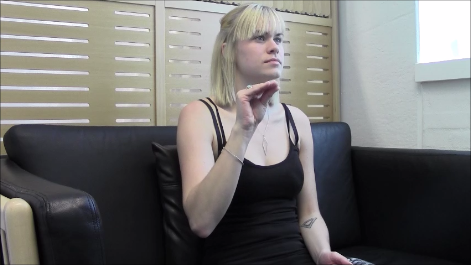
\includegraphics[resolution=300,width=0.9\textwidth]{FlowdiagramTest2/Test2_pause}
	\caption{Illustration af hvordan optagelsen foretages, med en 45$^\circ$'s vinkel i et halvnært perspektiv og hvor demonstratoren er siddende med et neutralt ansigtsudtryk.}
	\label{fig:Test2Pause}
\end{figure}
\noindent
%
Under optagelsen afspilles der musik fra en computer. Musiknummeret til at pause og starte musikken er "Love you can save it all" fra Andra (2016), musiknummeret der skiftes til, når der skiftes sang er "How would you feel" fra Ed Sheeran (2017) og musiknummeret til at skrue op og ned for musikken er "New man" fra Ed Sheeran (2017). Disse musiknumre er valgt ud fra de samme kriterier, som er beskrevet i \fullref{VideooptagelserValgAfGestikker}.

Optagelsen redigeres i Windows Movie Maker version 2012. På \autoref{fig:FlowdiagramFami} illustreres rækkefølgen på de skærmbilleder, som videoen består af.      
%
\begin{figure}[H]
	\centering
	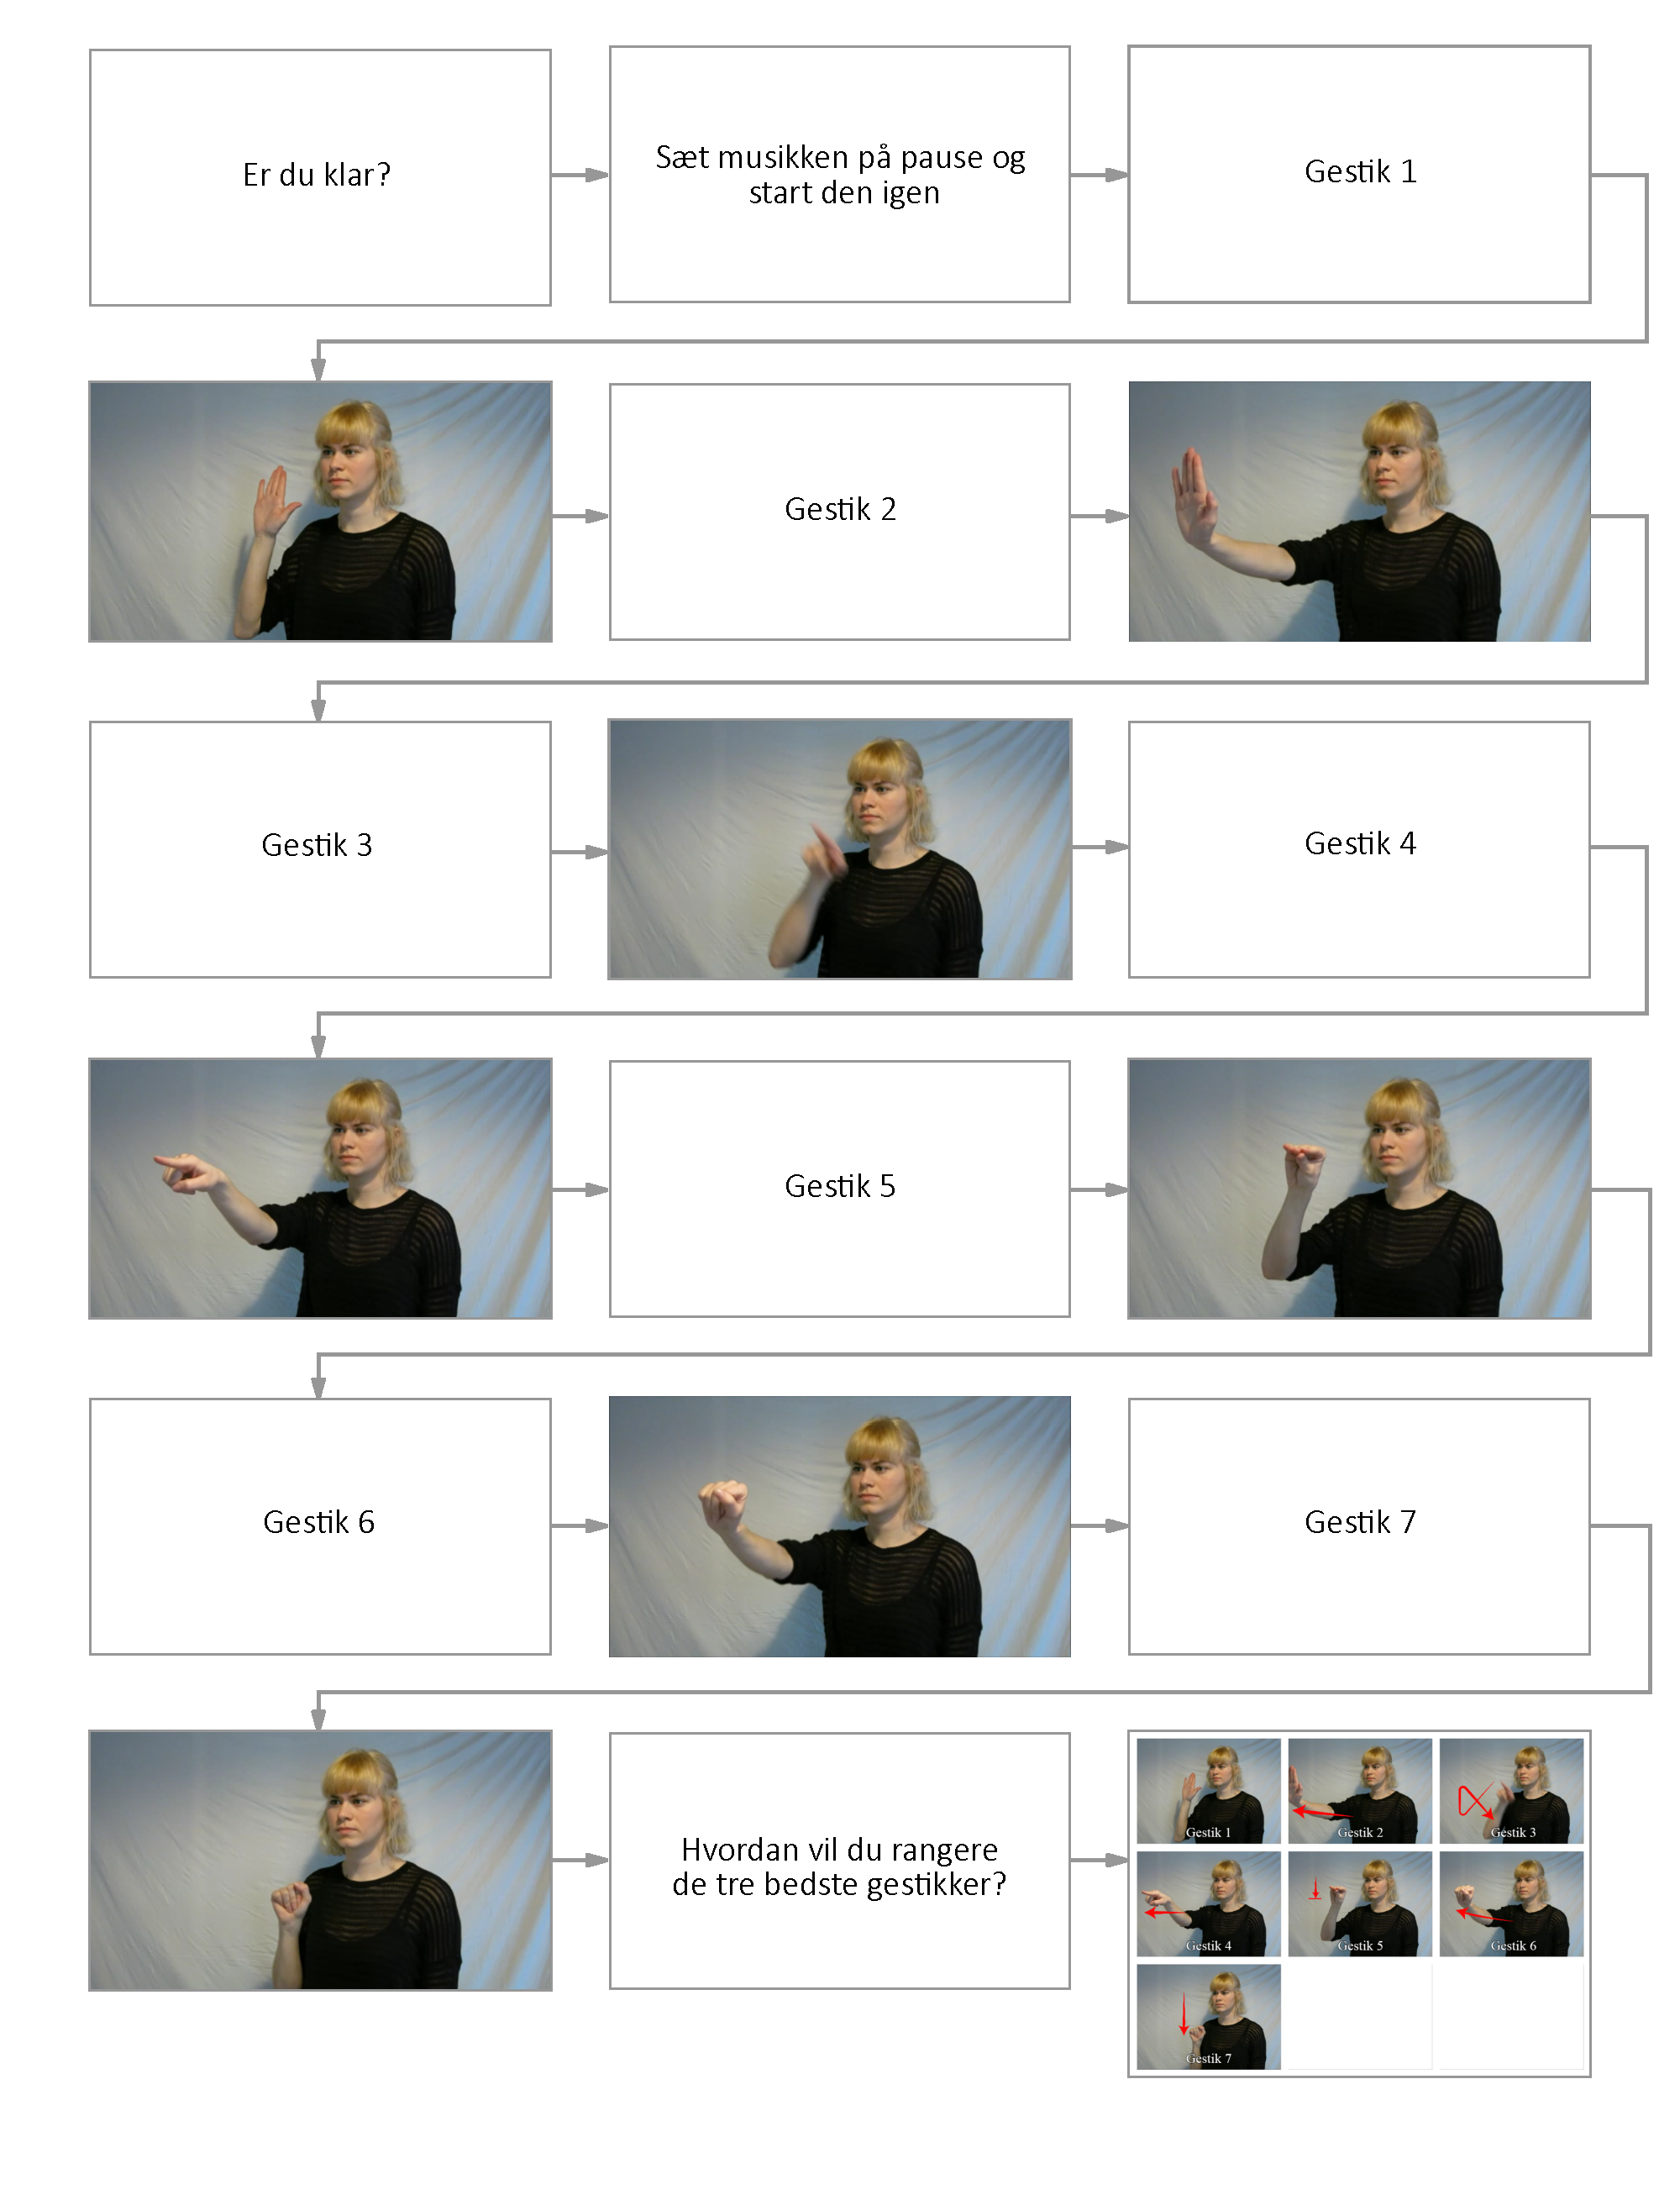
\includegraphics[resolution=300,width=\textwidth]{Flowdiagram/FlowdiagramPauseogStart}
	\caption{Illustration af hvilke skærmbilleder, der indgår i videoen til familiariseringen af værten.}
	\label{fig:FlowdiagramFami}
\end{figure}
\noindent
%
Det første skærmbillede testpersonerne præsenteres for består af teksten: \textit{Er du klar?} og præsenteres i 3 sekunder, før skærmbilledet med teksten: \textit{Sæt musikken på pause og start den igen} præsenteres i tre sekunder. Teksten på det andet skærmbillede tilpasses afhængigt af hvilken funktion, der præsenteres. Første gang testpersonerne præsenteres for de tre tekster, som angiver funktion, er varigheden tre sekunder kontra når testpersonerne præsenteres for de tre tekster anden gang, hvor varigheden sættes ned til to sekunder. Når testpersonerne er blevet præsenteret for hvilken gestik, der skal bruges til at skrue op og ned for musikken, er der et blankt skærmbillede på to sekunder, inden testpersonerne præsenteres for gestikkerne uden information omkring funktion. De to blanke skærmbilleder før og efter optagelsen af gestik-par 5 til at skifte musiknummer, varer et sekund. Efter optagelsen af gestik-par 2 til at skrue op og ned for musikken præsenteres endnu et blankt skærmbillede på to sekunder, hvorefter testpersonen er nået til den del af familiariseringen hvor de præsenteres for gestikkerne og derefter skal angive hvilken funktion gestikken tilhører. Skærmbilledet med teksten: \textit{Hvilken funktion havde gestikken?} præsenteres i syv sekunder og teksten tilpasses afhængigt af funktion. Alt i alt varer videoptagelsen 3 minutter og 16 sekunder. 